\chapter{Krótki start}
Poniżej opisano prosty przypadek użycia aplikacji, w którym dodano nowego właściciela do systemu, następnie nowe mieszkanie, a na końcu przypisano właściciela do tego mieszkania.

\noindent \textbf{Logowanie i panel główny~~}
Aby skorzystać z systemu należy się do niego zalogować. Na rysunku~\ref{fig:logowanie} przedstawiono panel logowania do świeżo uruchomionego systemu w środowisku Docker. Dane do logowania, takie jak e-mail i hasło super administratora, są konfigurowane w pliku \texttt{docker-compose.yml}. Jak widać na wspomnianym rysunku, do logowania użyto danych: \textbf{daniel.hhn.SA@gmail.com} oraz \textbf{superadmin\_password123}. Po udanym logowaniu system przeniesie użytkownika na panel główny pracownika pokazany na rysunku~\ref{fig:widoki}a.\\[-10pt]
\begin{figure}[ht]
	\centering
		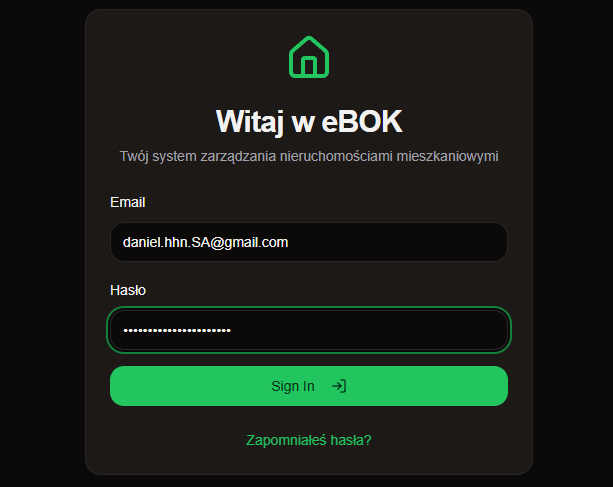
\includegraphics[scale=.6]{rys0C/logowanie_do_systemu}
		\caption{Logowanie do systemu jako super administrator}
	\label{fig:logowanie}
\end{figure}

\noindent \textbf{Dodanie nowego użytkownika do systemu~~}
Na panelu pracownika (rys.~\ref{fig:widoki}a), po lewej stronie widoczne są różne opcje do wyboru. Zawartość wyświetlana w części centralnej zależy wybranej opcji. W przypadku wybrania \texttt{Użytkownicy}, w części centralnej pojawi się zakładka zarządzania użytkownikami (rys.~\ref{fig:widoki}b), zaś w przypadku wybrania opcji \texttt{Mieszkania} -- zakładka do zarządzania mieszkaniami (rys.~\ref{fig:widoki}c).
Dodawanie nowego użytkownika można zrealizować na zakładce zarządzania użytkownikami. Wystarczy kliknąć na zielonym przycisku \texttt{Dodaj Użytkownika}. W reakcji na to kliknięcie otworzy się formularz, na którym można wprowadzić dane użytkownika, takie jak imię, nazwisko, e-mail, numer telefonu, hasło oraz rolę (rys.~\ref{fig:widoki}d). W omawianym przypadku należy wybrać rolę \texttt{ROLE\_OWNER}, co jest potrzebne by wykonać kolejny krok.
\begin{figure}[htb]
	\centering
  \begin{tabular}{@{}l@{}}
		a) \\  \vtop{\vskip-2ex\hbox{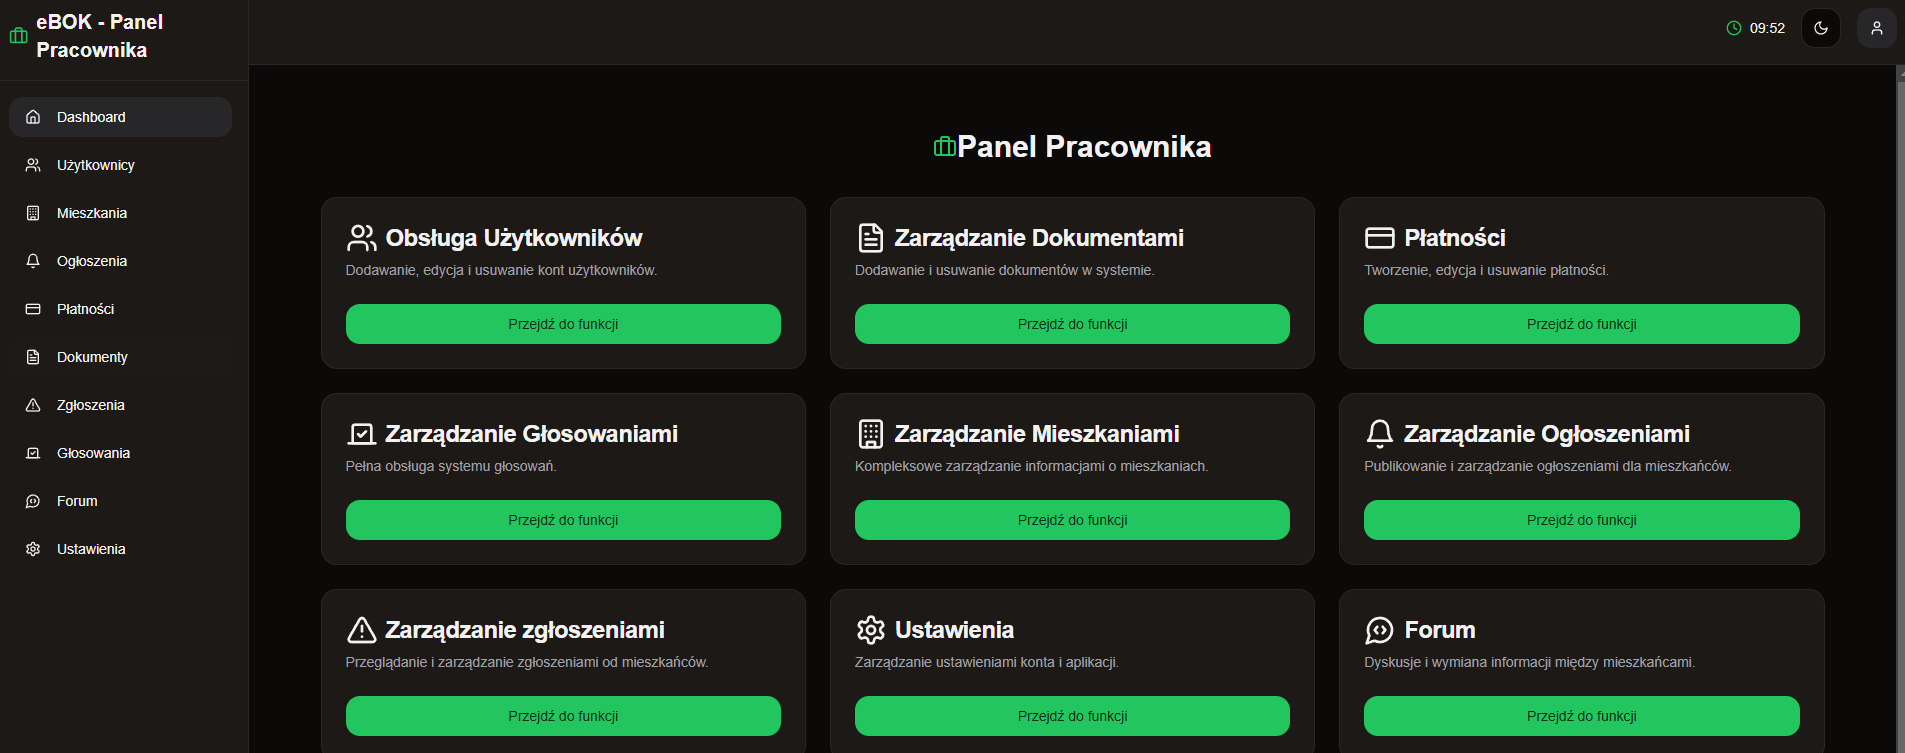
\includegraphics[width=\linewidth]{rys0C/panel_glowny_pracownika}}}\\
		b) \\  \vtop{\vskip-2ex\hbox{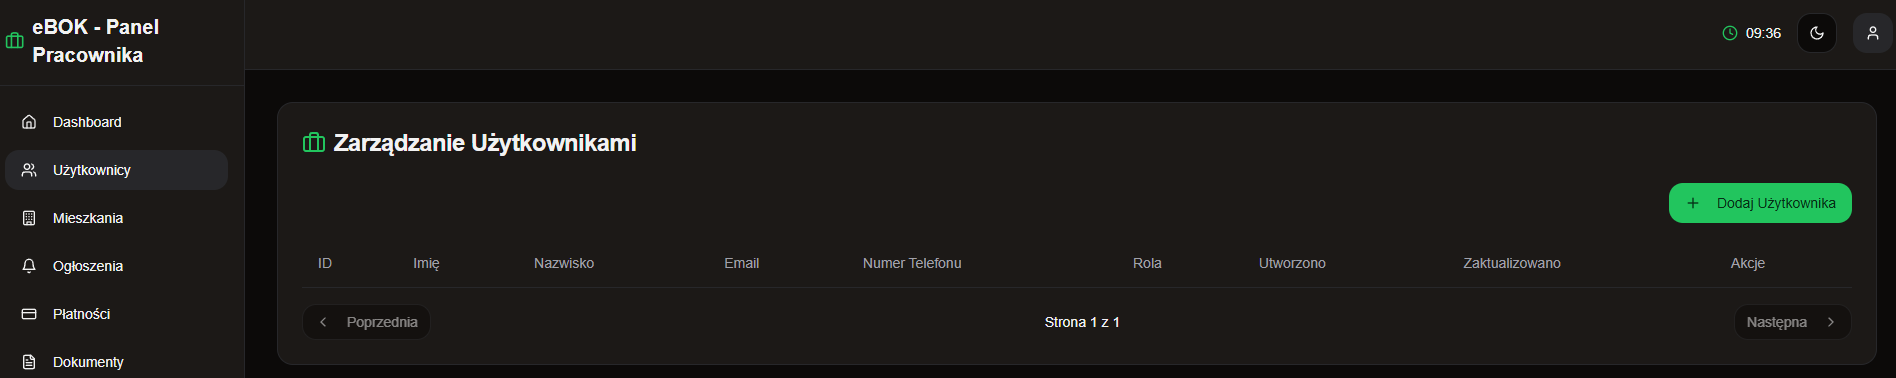
\includegraphics[width=\linewidth]{rys0C/zoskladka_do_uzytkownikow}}}\\
		c) \\ \vtop{\vskip-2ex\hbox{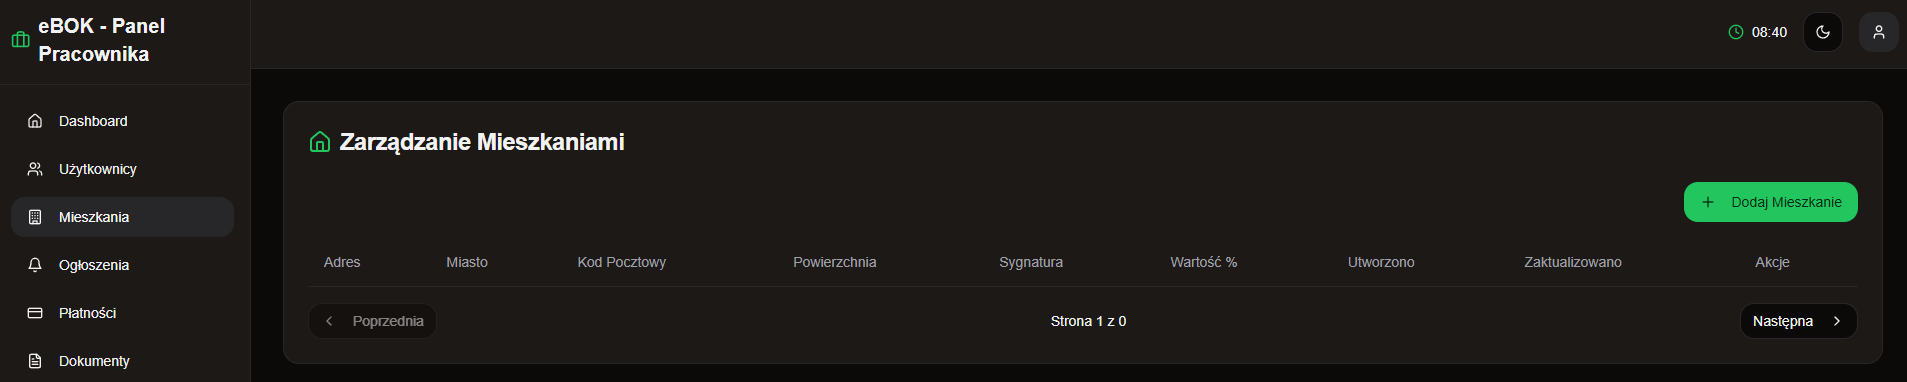
\includegraphics[width=\linewidth]{rys0C/zakladka_od_mieszkan}}} \\
		{\begin{tabularx}{\linewidth}{@{}XX@{}}
		d) &   e) \\
		\vtop{\vskip-2ex\hbox{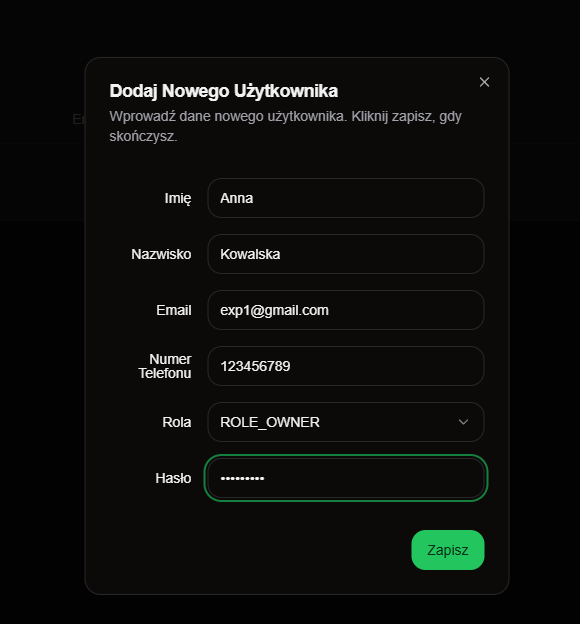
\includegraphics[scale=.6]{rys0C/dodanie_wlasciela}}} &
		\vtop{\vskip-2ex\hbox{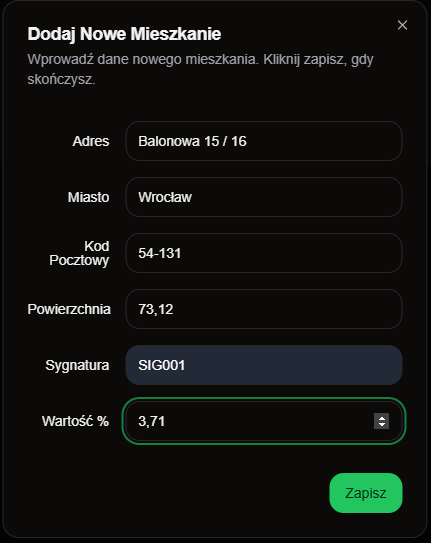
\includegraphics[scale=.6]{rys0C/dodanie_nowego_mieszkania}}}
		\end{tabularx}}
  \end{tabular}
		\caption{Widoki aplikacji: a) panel główny pracownika, b) zakładka zarządzania użytkownikami, c) zakładka zarządzania mieszkaniami}
	\label{fig:widoki}
\end{figure}
\clearpage

%\begin{figure}[htb]
    %\centering
    %\begin{tabular}{ll}
		%a) &   b) \\
		%\vtop{\vskip-2ex\hbox{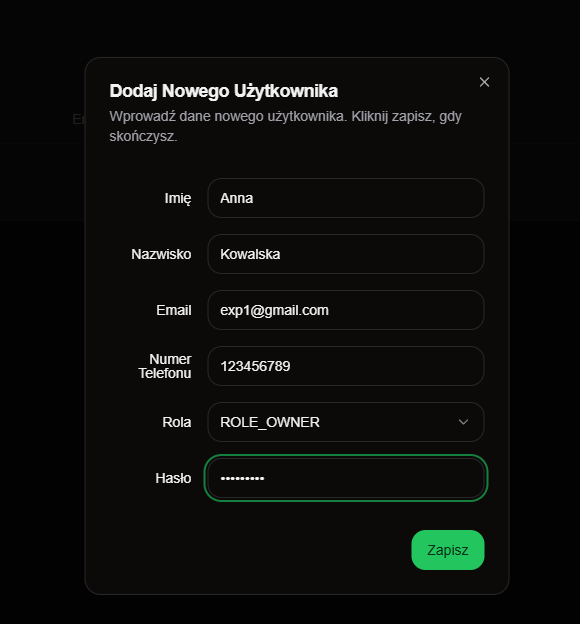
\includegraphics[scale=.6]{rys0C/dodanie_wlasciela}}} &
		%\vtop{\vskip-2ex\hbox{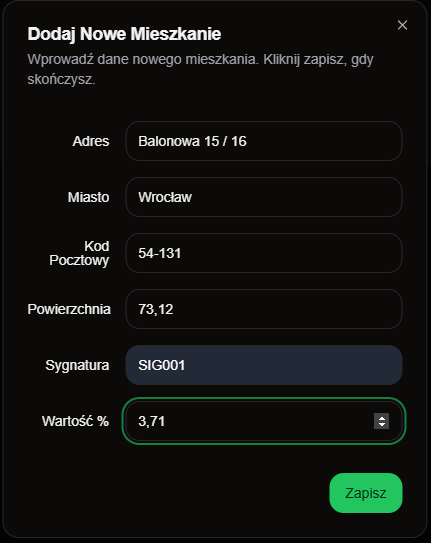
\includegraphics[scale=.6]{rys0C/dodanie_nowego_mieszkania}}}
		%\end{tabular}
    %\caption{Formularze dodawania: a) nowego użytkownika, b) nowego mieszkania}
    %\label{fig:add}
%\end{figure}


\noindent \textbf{Dodanie nowego mieszkania do systemu~~}
Aby dodać nowe mieszkanie, należy przejść do wspomnianej zakładki \texttt{Mieszkania}. Po tej czynności w części centralnej pojawi się Panel zarządzania mieszkaniami (rys.~\ref{fig:widoki}c). Kliknięcie na zielonym przycisku \texttt{Dodaj Mieszkanie} występującym na tej zakładce spowoduje wyświetlenie  formularza dodawania mieszkania (rys.~\ref{fig:widoki}e). W formularzu należy uzupełnić takie dane, jak adres, miasto, kod pocztowy, powierzchnia, sygnatura oraz procent udziału w nieruchomości.

\noindent \textbf{Przypisanie użytkownika do mieszkania~~} Po zakończeniu procesu dodawania nowego mieszkania zostanie ono uwidocznione na liście jak pokazano na rysunku~\ref{fig:apartment}a. Bezpośrednio po dodaniu mieszkanie nie będzie miało przypisanych właścicieli.
Aby tę sytuację zmienić należy przypisać właściciela do mieszkania. W tym celu należy na zarządzania mieszkaniami (rys.~\ref{fig:apartment}a) wybrać opcję \texttt{Przypisz Użytkownika} dostępną w kolumnie \texttt{Akcje}. Po wybraniu tej opcji otworzy się okienko (rys.~\ref{fig:apartment}b), w którym należy podać identyfikator użytkownika (\texttt{ID}) (to miejsce na identyfikator użytkownika dodanego wcześniej do systemu jako właściciel). Po pomyślnym przypisaniu właściciela system wyświetla zaktualizowaną listę właścicieli, jak przedstawiono na rysunku~\ref{fig:apartment}c.

\begin{figure}[htb]
    \centering
    \begin{tabular}{@{}l@{}}
		a) \\  \vtop{\vskip-2ex\hbox{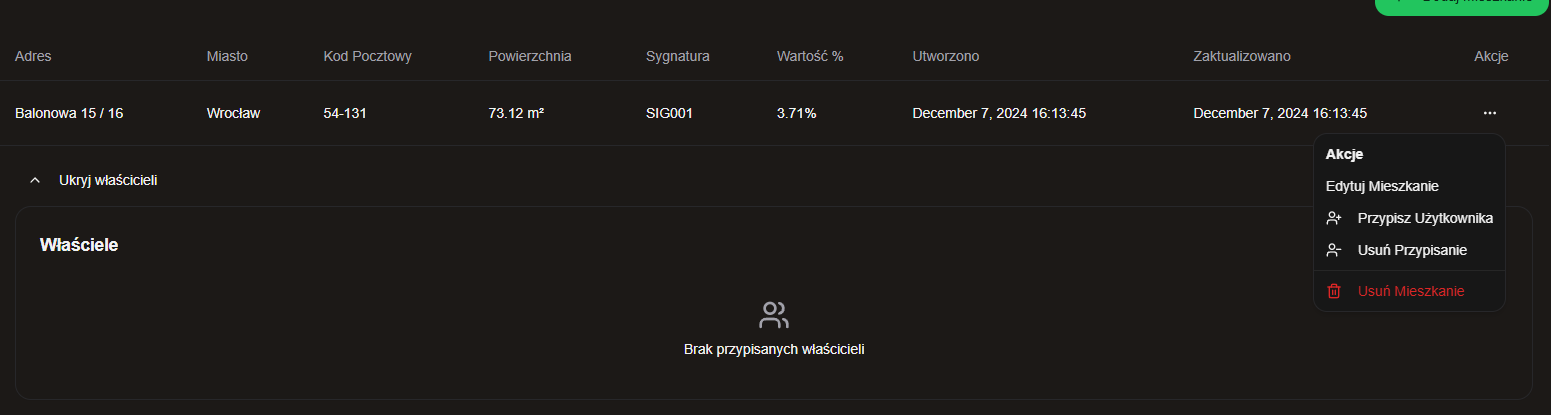
\includegraphics[width=\linewidth]{rys0C/jak_dodac_wlasciciela_1}}} \\
		b) \\  \vtop{\vskip-2ex\hbox{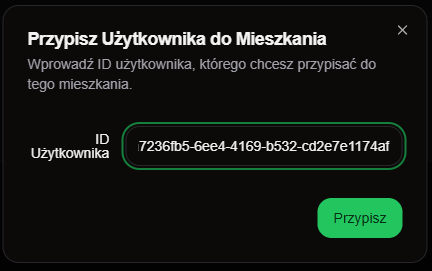
\includegraphics[scale=.55]{rys0C/jak_dodac_wlasciciela_2}}} \\
    c) \\  \vtop{\vskip-2ex\hbox{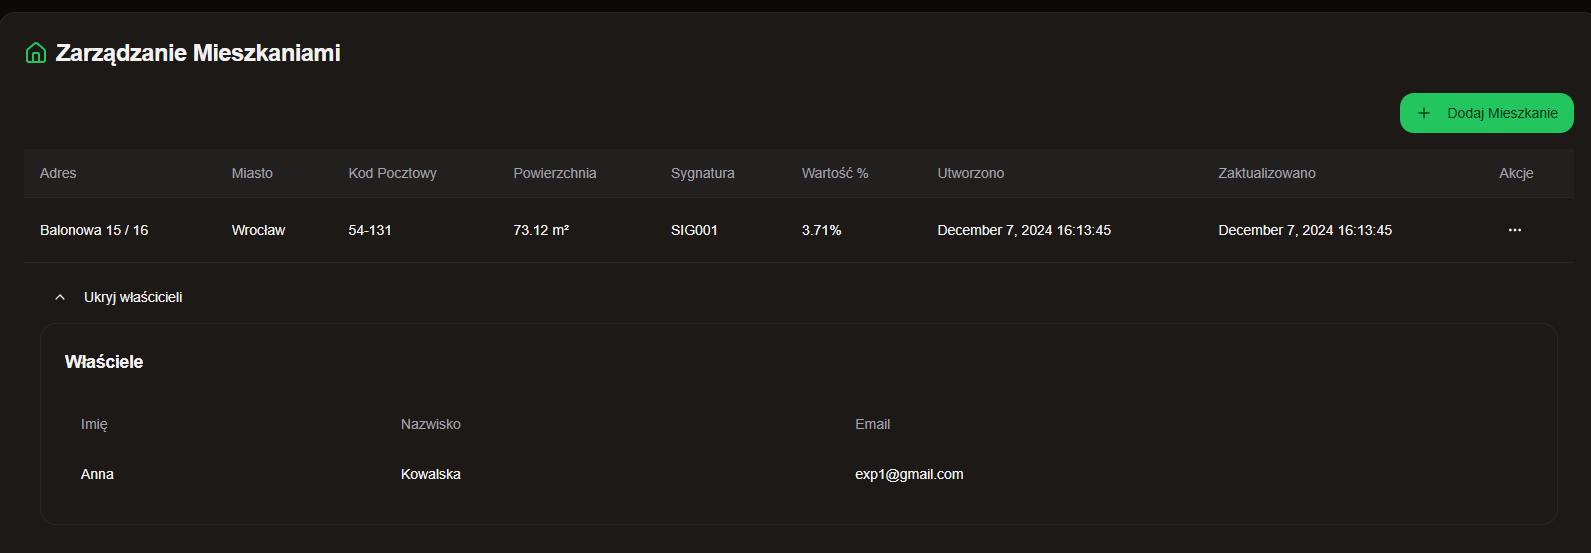
\includegraphics[width=\linewidth]{rys0C/wlasciciel_dodany}}}
		\end{tabular}
    \caption{Dodawanie nowego mieszkania: a) dane nowego mieszkania bez przypisanego właściciela, b) przypisywania właściciela do mieszkania, c) wynik udanego przypisanie właściciela do mieszkania}
    \label{fig:apartment}
\end{figure}


